In this section, we will first describe our data-collection process. Next we will show the code repair, and detection accuracy techniques on a small subset of this collected dataset.   

\subsection{Data collection} 
  We used dataset from two previous sources ~\cite{meng2018secure,fischer2017stack}. Both of these dataset contain code snippets posted on Stackoverflow. 
  Fisher et al. crawled 1,161 code snippets posted on Stackoverflow related to Andrioid Securuity ~\cite{fischer2017stack}. They considered a code snippet related to Android security if the code snippets makes API calls to
  one of the security services such as Java cryptography, Java secure Communications, public key infrastructure X.509 certificates, and Java authentication - authorization services. The popular crypto libraries used by Andriod developers such as Bouncy Castle, SpongyCastle, Apache TLS/SSL, keyczar, jasypt, and GNU Crypto were also included. 
  
  Meng et al.  extracted 503 code snippets from 22,195 Stackoverflow posts by filtering the posts based on votes, duplications, and absence of code snipeets~\cite{meng2018secure}. In total our study is baded on the dataset by combining these two. Our dataset contains 1,664 code snippets. The timeline of these code snippets are from 2008-2017.
  \minote{add some more info and some statistics}

  As to get the ground truth of the presence of insecure pattern, we have to manully analysis them, it becomes very time consuming. Therefore to make the analysis less consuming time , we only consider randomly sampled 800 code snippets -- about half of the 1.6K code snippets available. 
  We then assign the code snippets into one of the 8 insecure patterns.  %and record the common keywords appear in the code snippets. By doing this we have list of common keyword for each of the 8 insecure patterns. We can then categorize all 1.6K code snippets using these common keywords.
  

\subsection{Code repair success rate.} 
%AES: 85/225 Broken-Hash: 69/219 
% Constructor class
\begin{figure}[ht]
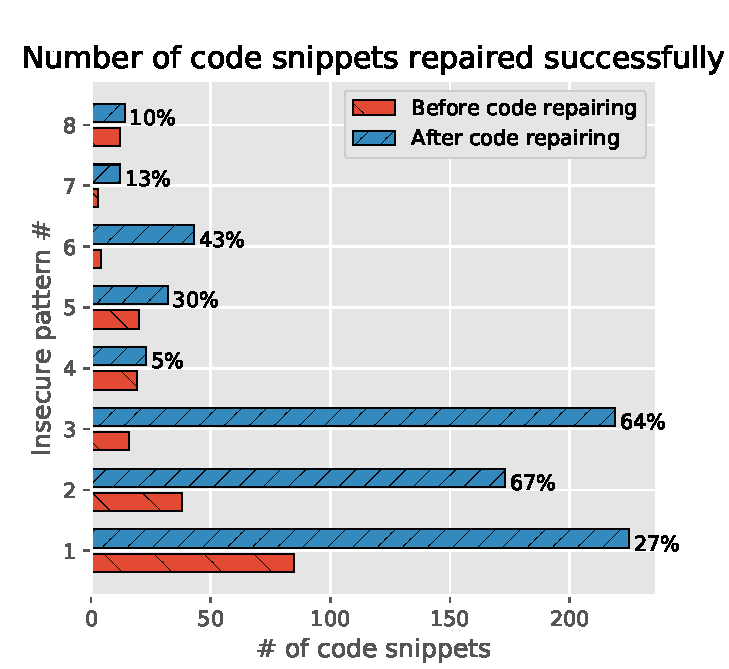
\includegraphics[width=\linewidth]{Figures/success_full_repair2.eps-eps-converted-to.pdf}
\caption{Percentage of code snippets successfully repaired.}
\label{fig:code-repair}
\end{figure}

We called a code snippet successfully repaired if we can convert it to a Jimple IR. Figure~\ref{fig:code-repair} illustrates the percentage of code snippets for each categorize, we have been able to parsed (i.e., convert to Jimple IR), using the code repair techniques discussed in subsection~\ref{subsec:code-repair}.  
\subsection{Insecure pattern detection accuracy.}
After converting each successfully repaired code snippets to Jimple IR, we detected rule 7, and 8 using keyword searching as mentioned previously. However for rule 1-6, need to apply backword flow analysis. To do this we give the Jimple IR to our tool. Out tool is built on top of CryptoGurd. CryptoGurd uses Soot as its program analysis enginee. Using Soot's \texttt{JimpleAST} API~\footnote{\url{https://www.sable.mcgill.ca/soot/doc/soot/jimple/parser/JimpleAST.html}}, we can enable backword flow analysis given the slicing criteria from Table~\ref{tab:slicing}. The idea is track the special method invokations parameter from the slicing criteria. In this way we can inspect the set of program statements which are affected by this slicing criteria and figure out the presence of insecure patterns. 


Table~\ref{tab:results} shows the total number of code snippets for of the 8 rules (they sum up to more than 800 as some code snippets has two or more rules). Parsed column refers to the number of code snippets, we have been able to convert to Jimple IR after applying the code repair discussed in section~\ref{subsec:code-repair}. We also shows the TP, FN, FN along side the precision, and recall.
As it can seen we have not been able to run backword flow analysis for rule 3. The reasons are explain the in the appendix.
%If any of these set of program statements contains i) 
% Say you have done the  1,2,4,5, 7,8 correctely. How to present the results? 
% say you haven trying to address the problem of empty method detection but have not been able to do so. 


\begin{table}[ht]
\begin{tabular}{|l|r|r|r|r|r|r|r|}
\toprule
Rule no & Total & Parsed & TP & FP & FN & Precision & Recall \\ \midrule
1 & 225 & 85 & & & &  & \\
2 & 173 & 38 & & & & & \\
3 & 219 & 69 & - & - & - & - & - \\
4 & 68 & 19 &  & & & & \\
5 & 40 & 24 & & & & & \\
6 & 90 & 12 & & & & & \\ \midrule
7 & 68 & 24 & & & & &\\
8 & 20 & 10 & & & & &\\        
\bottomrule
\end{tabular}
\caption{Table}
\label{tab:results}
\end{table}